\documentclass{article}\usepackage[]{graphicx}\usepackage[]{xcolor}
% maxwidth is the original width if it is less than linewidth
% otherwise use linewidth (to make sure the graphics do not exceed the margin)
\makeatletter
\def\maxwidth{ %
  \ifdim\Gin@nat@width>\linewidth
    \linewidth
  \else
    \Gin@nat@width
  \fi
}
\makeatother

\definecolor{fgcolor}{rgb}{0.345, 0.345, 0.345}
\newcommand{\hlnum}[1]{\textcolor[rgb]{0.686,0.059,0.569}{#1}}%
\newcommand{\hlsng}[1]{\textcolor[rgb]{0.192,0.494,0.8}{#1}}%
\newcommand{\hlcom}[1]{\textcolor[rgb]{0.678,0.584,0.686}{\textit{#1}}}%
\newcommand{\hlopt}[1]{\textcolor[rgb]{0,0,0}{#1}}%
\newcommand{\hldef}[1]{\textcolor[rgb]{0.345,0.345,0.345}{#1}}%
\newcommand{\hlkwa}[1]{\textcolor[rgb]{0.161,0.373,0.58}{\textbf{#1}}}%
\newcommand{\hlkwb}[1]{\textcolor[rgb]{0.69,0.353,0.396}{#1}}%
\newcommand{\hlkwc}[1]{\textcolor[rgb]{0.333,0.667,0.333}{#1}}%
\newcommand{\hlkwd}[1]{\textcolor[rgb]{0.737,0.353,0.396}{\textbf{#1}}}%
\let\hlipl\hlkwb

\usepackage{framed}
\makeatletter
\newenvironment{kframe}{%
 \def\at@end@of@kframe{}%
 \ifinner\ifhmode%
  \def\at@end@of@kframe{\end{minipage}}%
  \begin{minipage}{\columnwidth}%
 \fi\fi%
 \def\FrameCommand##1{\hskip\@totalleftmargin \hskip-\fboxsep
 \colorbox{shadecolor}{##1}\hskip-\fboxsep
     % There is no \\@totalrightmargin, so:
     \hskip-\linewidth \hskip-\@totalleftmargin \hskip\columnwidth}%
 \MakeFramed {\advance\hsize-\width
   \@totalleftmargin\z@ \linewidth\hsize
   \@setminipage}}%
 {\par\unskip\endMakeFramed%
 \at@end@of@kframe}
\makeatother

\definecolor{shadecolor}{rgb}{.97, .97, .97}
\definecolor{messagecolor}{rgb}{0, 0, 0}
\definecolor{warningcolor}{rgb}{1, 0, 1}
\definecolor{errorcolor}{rgb}{1, 0, 0}
\newenvironment{knitrout}{}{} % an empty environment to be redefined in TeX

\usepackage{alltt}

\usepackage{amsmath} %This allows me to use the align functionality.
                     %If you find yourself trying to replicate
                     %something you found online, ensure you're
                     %loading the necessary packages!
\usepackage{amsfonts}%Math font
\usepackage{graphicx}%For including graphics
\usepackage{hyperref}%For Hyperlinks
\usepackage[shortlabels]{enumitem}% For enumerated lists with labels specified
                                  % We had to run tlmgr_install("enumitem") in R
\hypersetup{colorlinks = true,citecolor=black} %set citations to have black (not green) color
\usepackage{natbib}        %For the bibliography
\setlength{\bibsep}{0pt plus 0.3ex}
\bibliographystyle{apalike}%For the bibliography
\usepackage[margin=0.50in]{geometry}
\usepackage{float}
\usepackage{multicol}

%fix for figures
\usepackage{caption}
\newenvironment{Figure}
  {\par\medskip\noindent\minipage{\linewidth}}
  {\endminipage\par\medskip}
\IfFileExists{upquote.sty}{\usepackage{upquote}}{}
\begin{document}

\vspace{-1in}

\title{Lab 5 Report -- Math240 -- Compuational Statistics}
\author{
  Jeremy Artiga \\
  Colgate University \\
  No Department \\
  {\tt{jartiga@colgate.edu}}
}

\date{}

\maketitle

\begin{multicols}{2}
\begin{abstract}
Music Analysis can be a daunting task which can take up hours, even days of your time! Thankfully, 
we have \texttt{R} and it's libraries to help us perform this music analysis. We will be analyzing
``Allentown" and it's contributing bands to find out who contributed more to the song.
\end{abstract}

\textbf{Keywords:} This lab will enable us to practice (1) utilizing libraries; (2) working with numerical
and character objects; (3) writing \texttt{for()} loops; (4) using \texttt{tidyverse} syntax; (5) summarize
data numerically and visually; (6) using \\ summaries to answer questions.

\section{Introduction}
The objective for this lab is to use \texttt{R} and it's libraries to figure out which band contributed most to the song ``Allentown": Manchester Orchestra, All Get Out, or The Front Bottoms? \\

\noindent To accomplish this, we will:
\begin{enumerate}
  \item Create batch files to process song data using Essentia.
  \item Use \texttt{jsonlite} \citep{jsonlite} to extract song data from processed \texttt{.JSON}
  files.
  \item Collect/Extract data from Essentia \citep{bogdanov2013essentia} and LIWC \citep{liwc22} models.
  \item Combine our Data into a Master data frame for analysis.
  \item Summarize/Analyze our data utilizing \texttt{tidyverse} \citep{tidyverse} and plots.
\end{enumerate}

\section{Methodology}

\subsection{Processing Song Data via Essentia Batch Files and Extracting Data Using \texttt{jsonlite}}
By utilizing packages and base \texttt{R} coding structures such as \texttt{for()} loops, objects, and accessing
elements within vectors/lists, we were able to create an Essentia command batch file from examination of 
\texttt{.WAV} files in the music directory. This not only enabled us to practice our abilities to utilize the said
coding structures, but it also allowed us to build an \texttt{R} program which could analyze any sort of directory
and pull the \texttt{.WAV} files for the sake of data processing into Essentia. We also figured out how to extract
data from .JSON files using the \texttt{jsonlite} package to gather information on specific albums/songs, which will
allow us to collect even more data which could be used in data analysis..

\subsection{Scaling up Data Extraction and Data Summarization via Boxplots}
The next step in accomplishing our objective is to upscale our data extraction process to collect data
from all the \texttt{.json} files we now possess from the music processing we did earlier in Essenita. By utilizing
the \texttt{jsonlite} package and \texttt{tidyverse}, we collected a variety of data points and built a data frame. We also furthered our data collection by extracting data from LIWC and Essenita models, which contain additional information on the songs we want to analyze. We constructed additional data frames using the same processes. By the end of this process, we were able to combine all of our data frames into a single ``Master" data frame using additional \texttt{R} functions, this will be used for our data analysis. \\
\noindent As a start to our data summary/analysis, we plotted three possible song traits between artists that could give us insights on our initial question (i.e. objective); Dissonance and Emotion (One sound and lyrical trait).

\subsection{Full Data Summary via \texttt{tidyverse} and More Plots}
The last task we need to perform to accomplish our objective is to summarize our data and analyze it using a plot. To do so, we will determine how similar Allentown is to each artist (Manchester Orchestra, All Get Out, The Front Bottoms) by song traits. To do this, we will do a mathematical version of the box plot and determine whether Allentown's traits is within range(similar), outlying(marginal), and out of range(not similar) using features in \texttt{tidyverse}. By Repeating this process for each song trait for each artist, we will be able to use \texttt{tidyverse} to combine the analyzed traits into a data frame. All we need to do now is to count the number of within ranges, outlying, and out of ranges for each artists and put them into a summarized data frame, this will be the data used for our column plots and table which will give us our answer to the initial question. 

\pagebreak

\end{multicols}

\section{Results}


% latex table generated in R 4.4.2 by xtable 1.8-4 package
% Thu Feb 27 17:17:41 2025
\begin{table}[H]
\centering
\begingroup\small
\begin{tabular}{lrrr}
  \hline
Artists & In Range & Outlying & Out of Range \\ 
  \hline
All Get Out & 166.00 & 17.00 & 14.00 \\ 
  Manchster Orchestra & 185.00 & 11.00 & 1.00 \\ 
  The Front Bottoms & 159.00 & 11.00 & 27.00 \\ 
   \hline
\end{tabular}
\endgroup
\end{table}


\begin{figure}[h]
  \begin{minipage}{0.35\textwidth}
    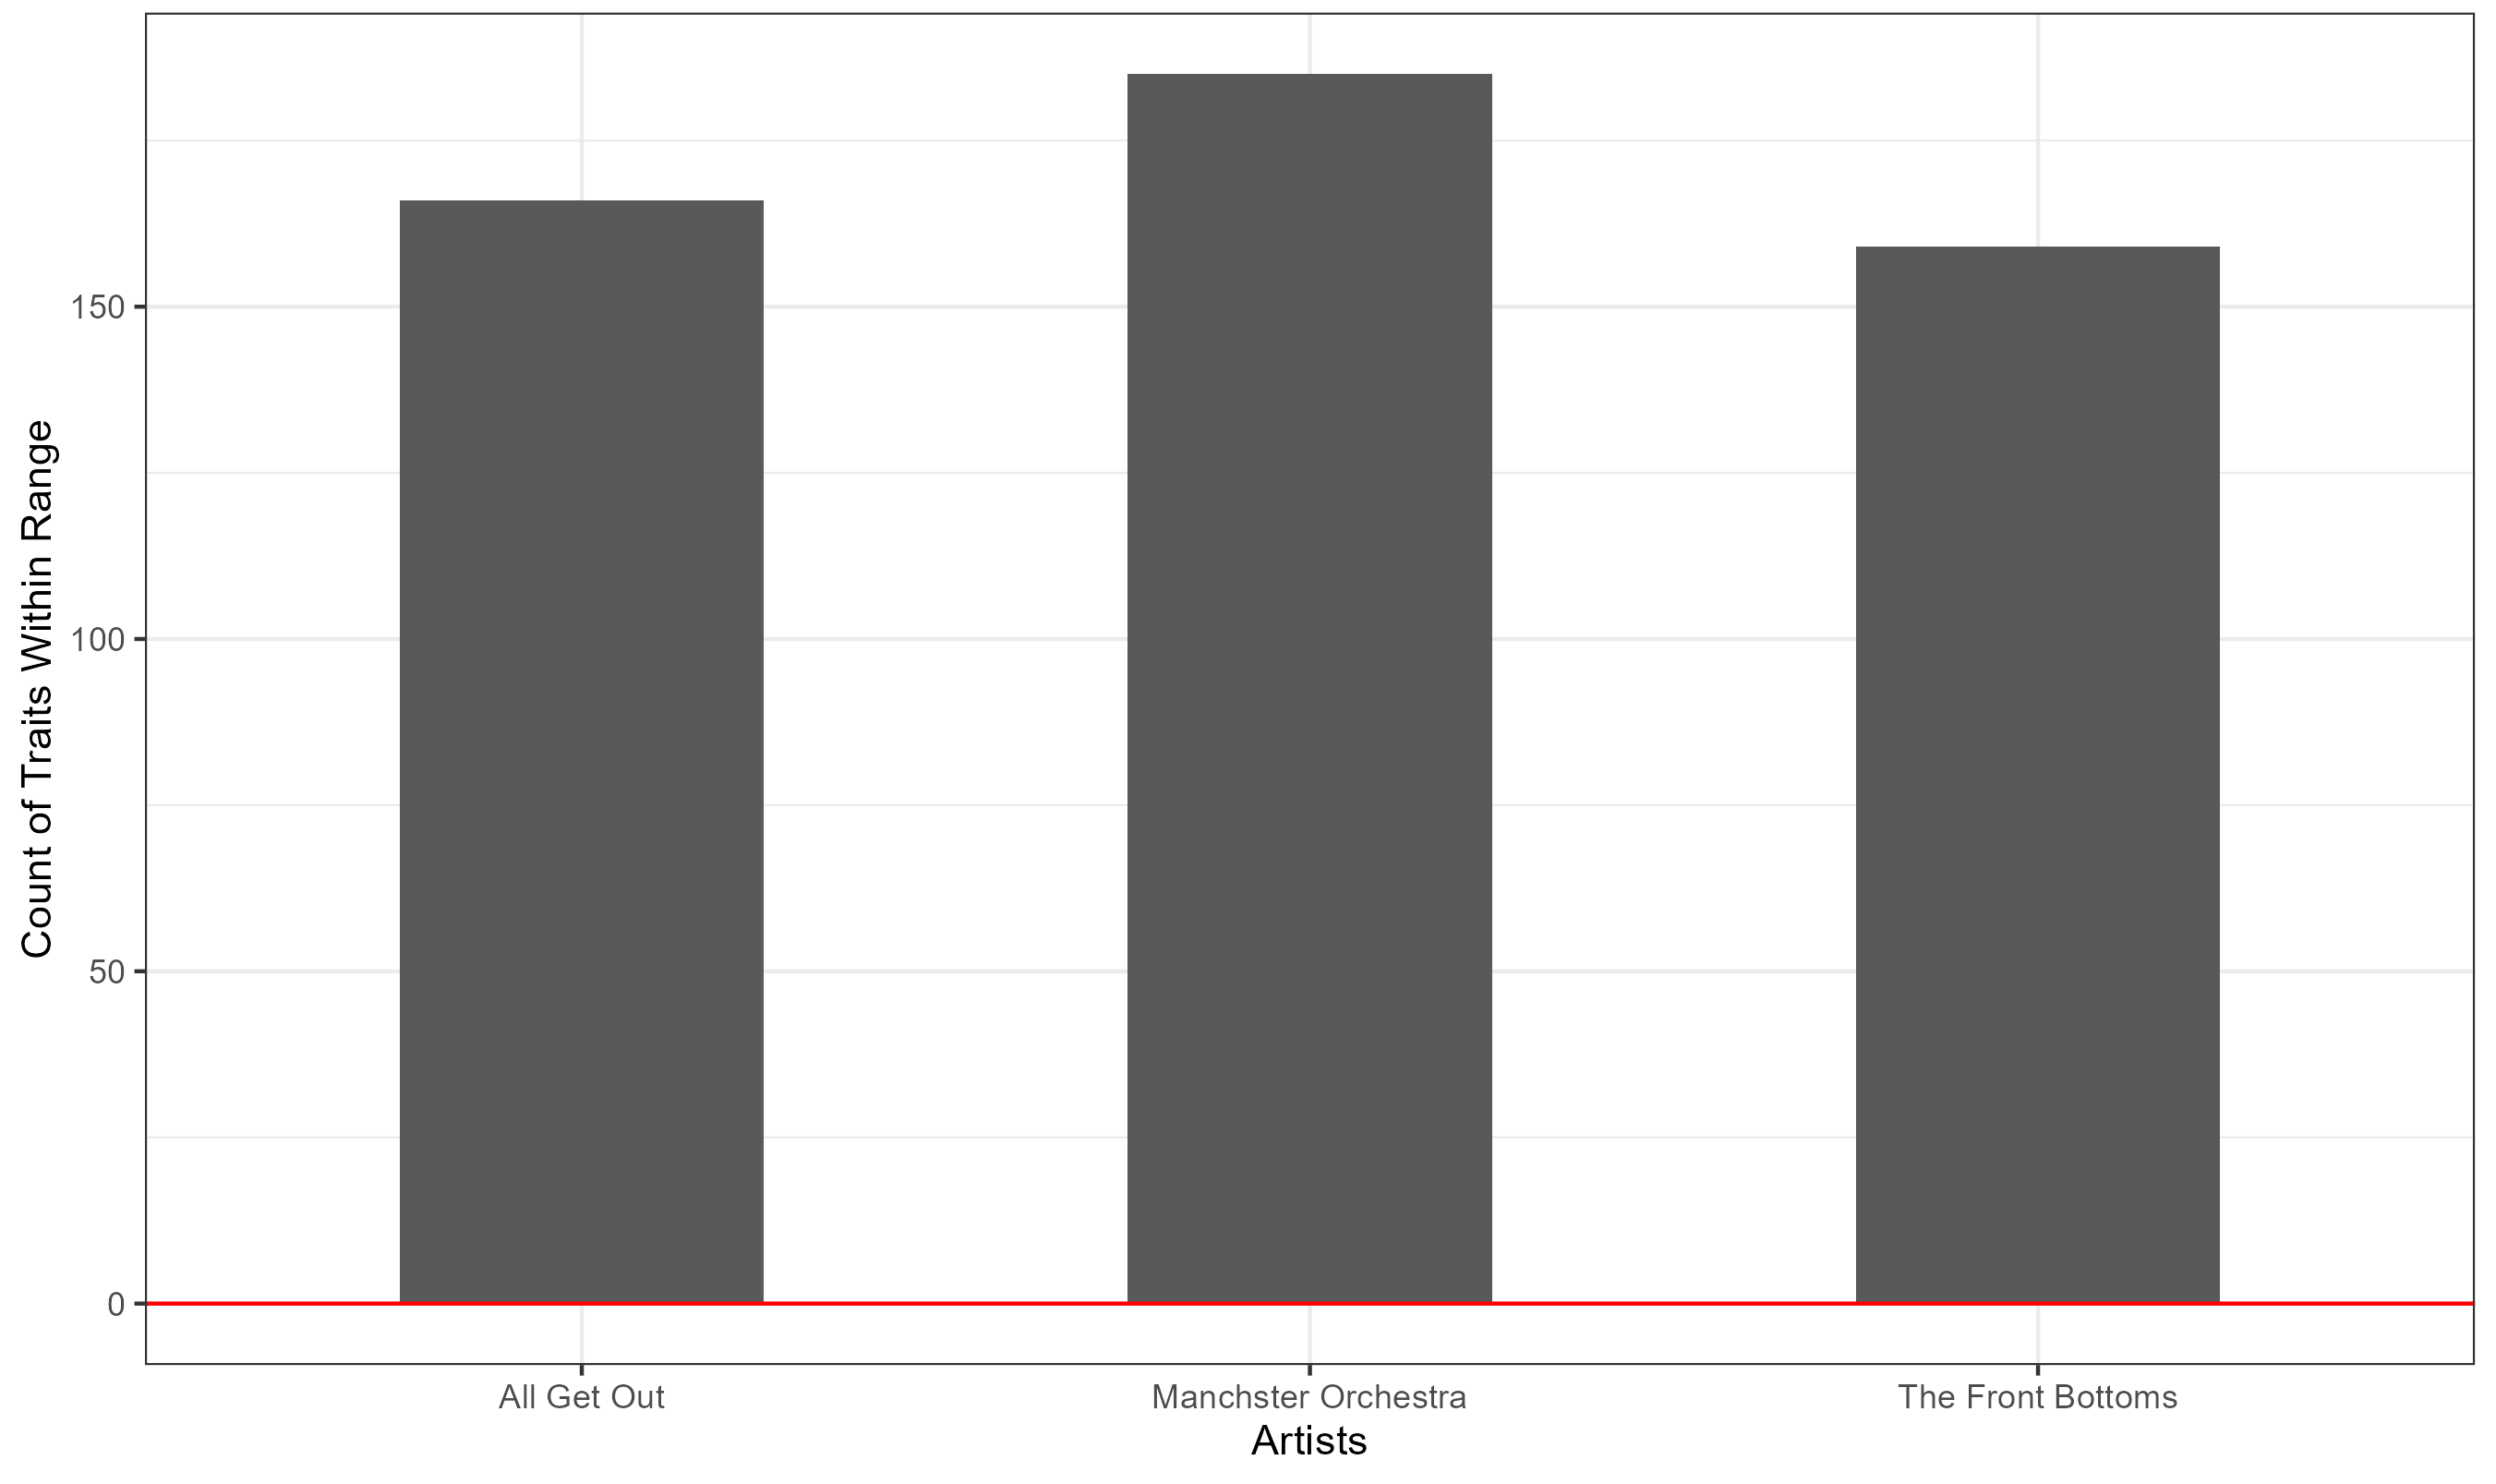
\includegraphics[width=\textwidth]{SimilarTraits.png}  
    \caption{Distribution by Similar Song \\ Traits}
    \label{fig:example}
   \end{minipage}
   \begin{minipage}{0.35\textwidth}
    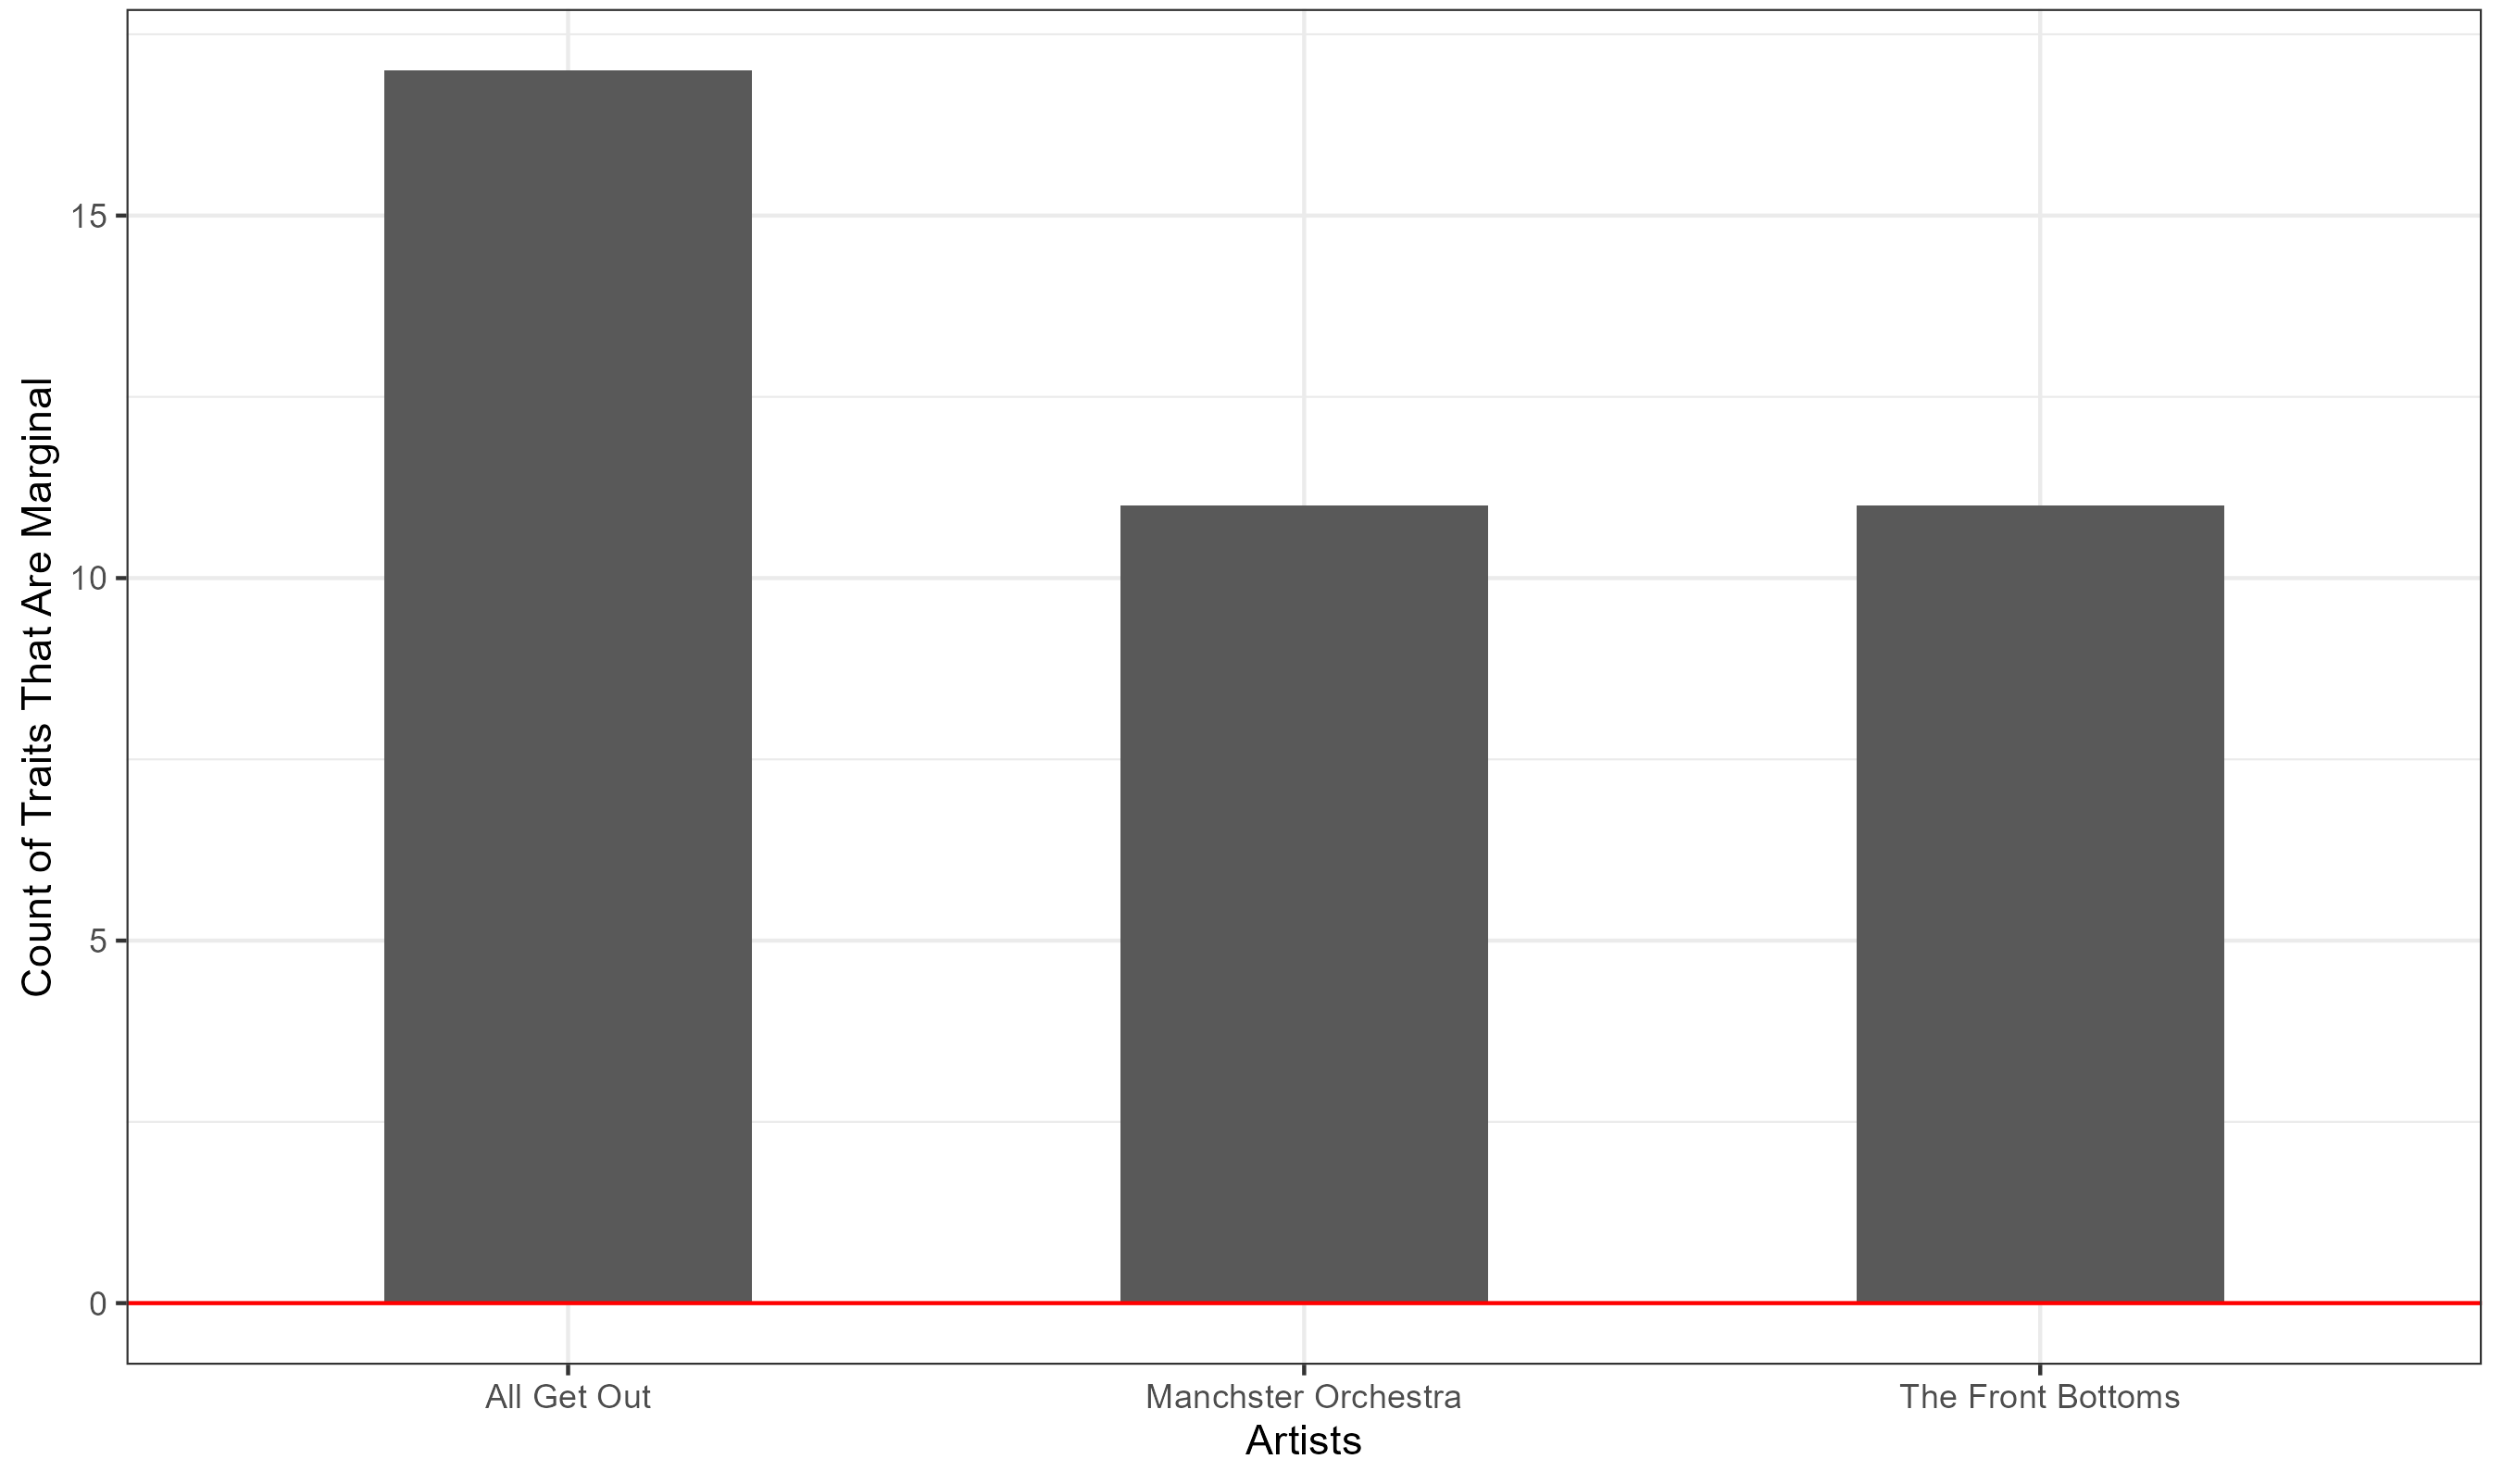
\includegraphics[width=\textwidth]{MarginalTraits.png}  
    \caption{Distribution by Marginal Song \\ Traits}
    \label{fig:example}
   \end{minipage}
   \begin{minipage}{0.35\textwidth}
    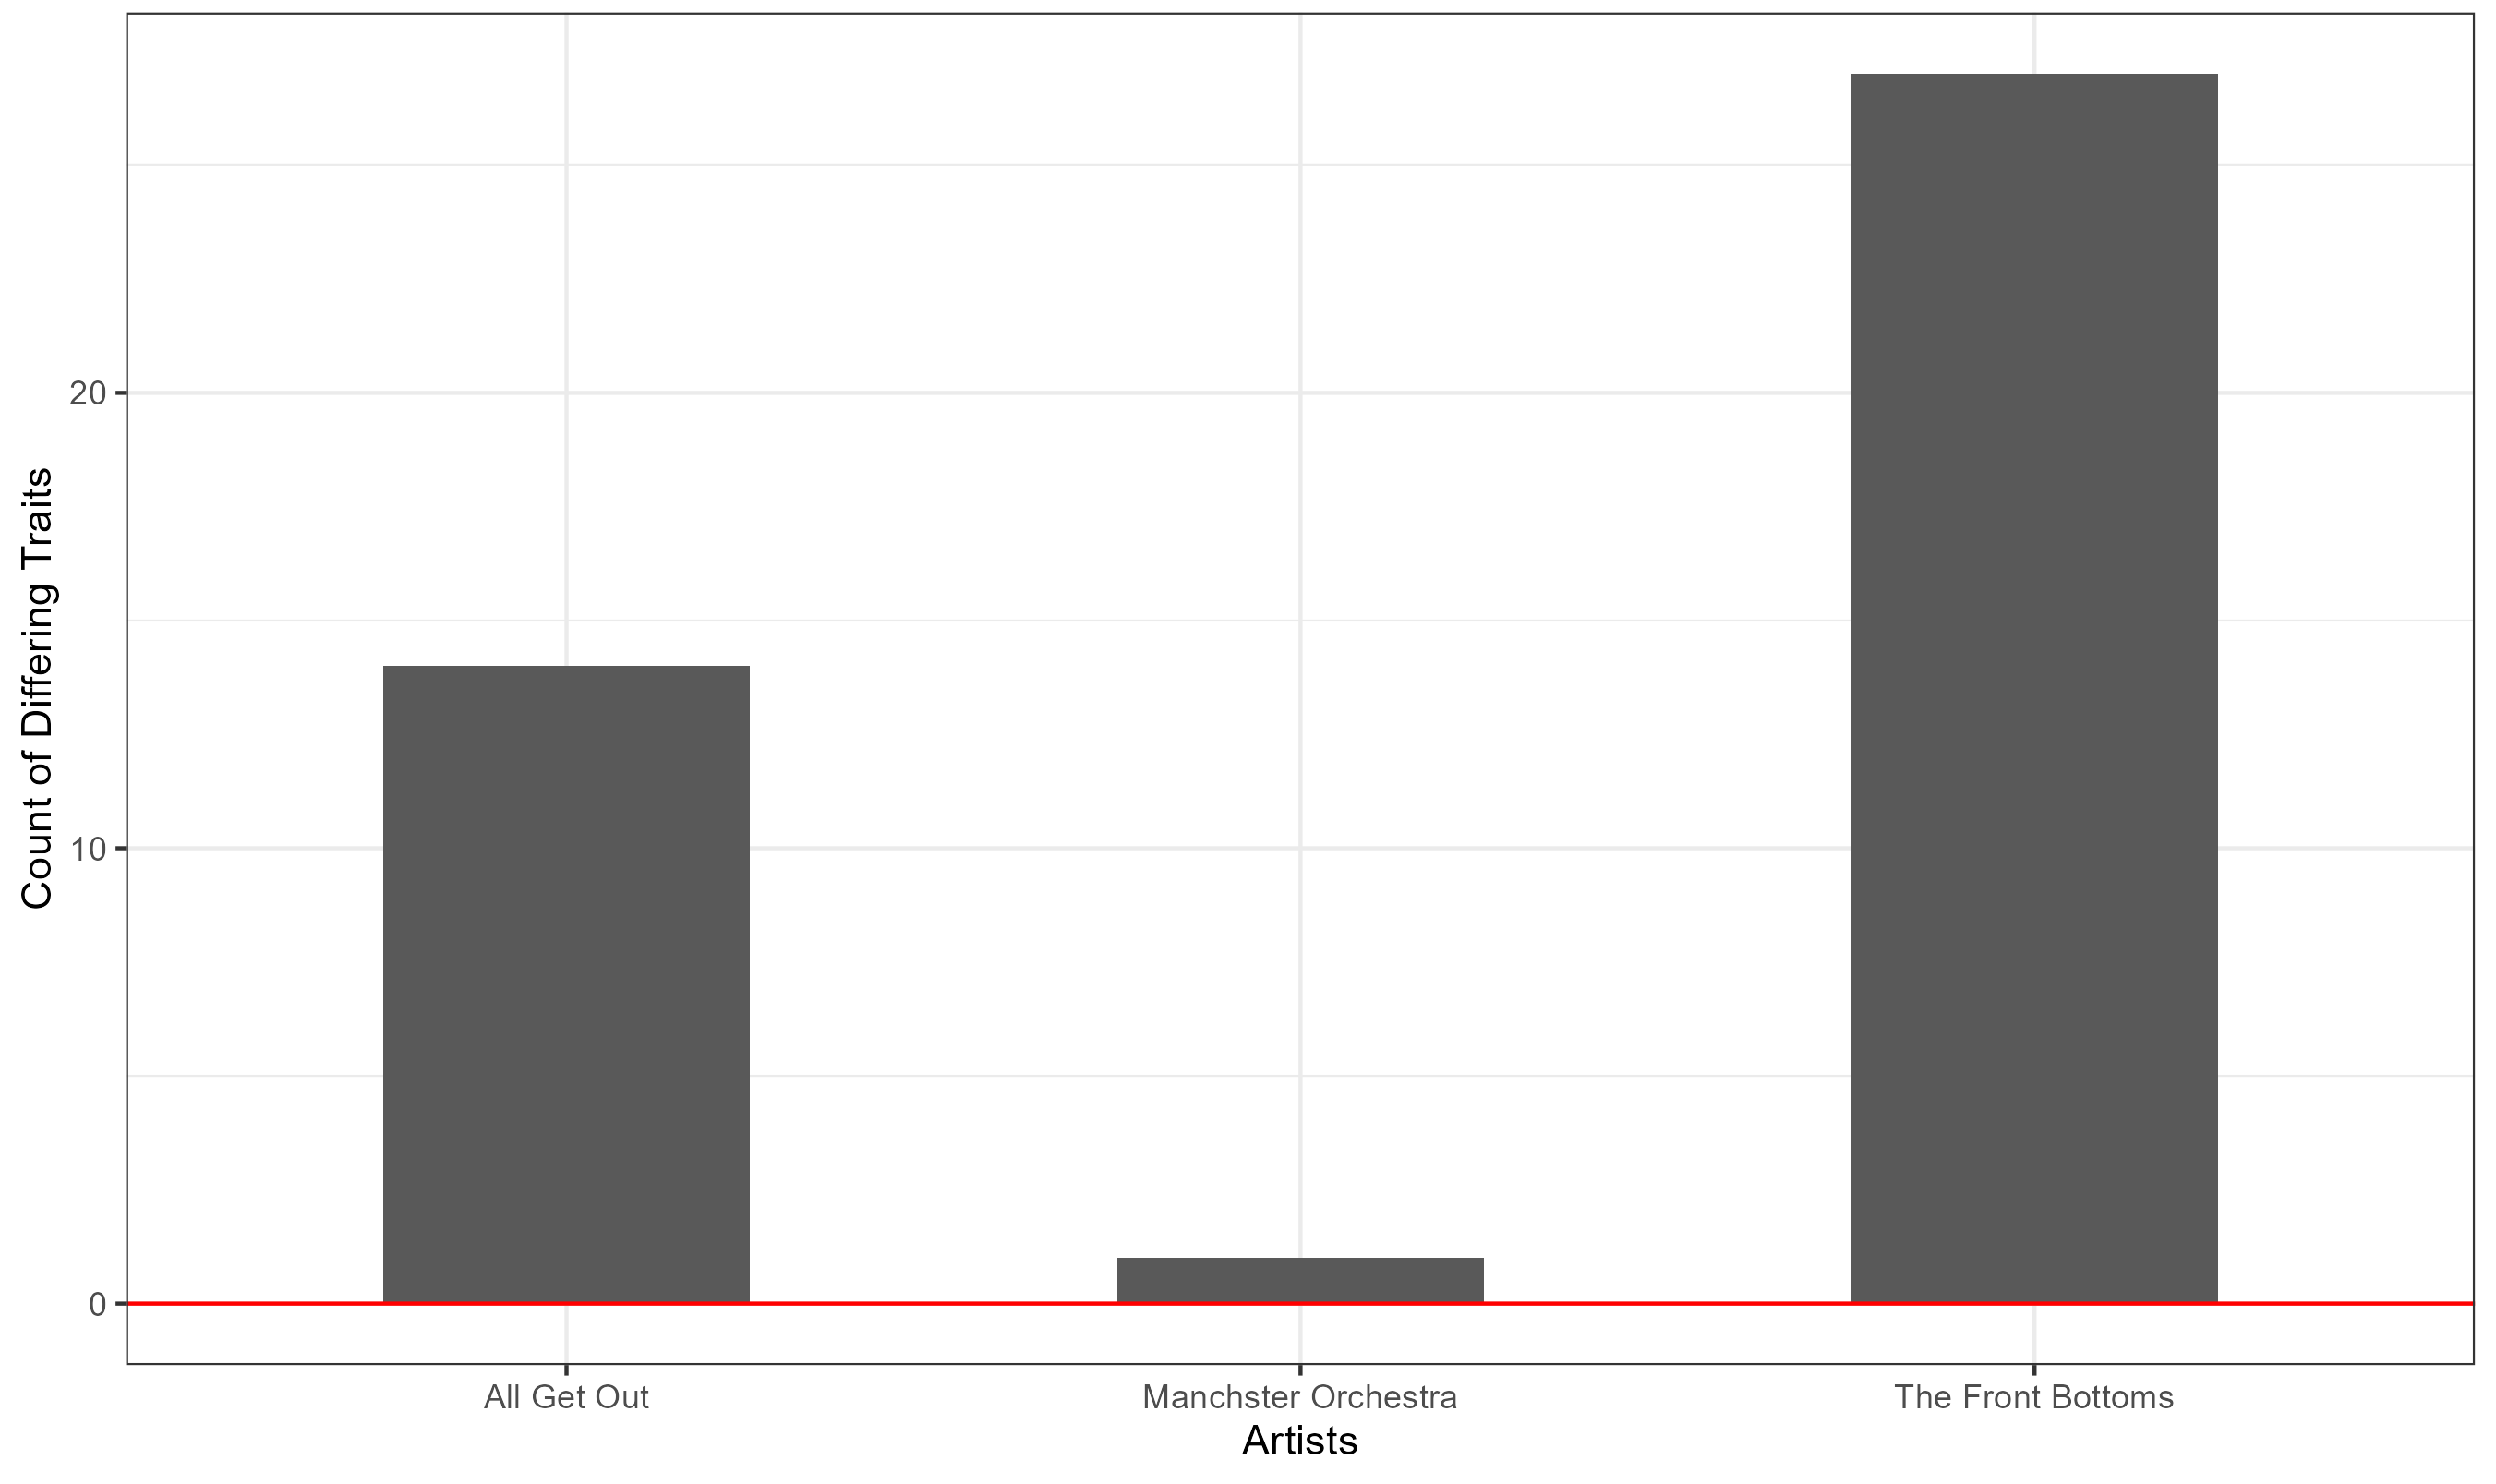
\includegraphics[width=\textwidth]{DifferentTraits.png} 
    \caption{Distribution by Different Song \\ Traits}
    \label{fig:example}
   \end{minipage}
\end{figure}

\begin{knitrout}
\definecolor{shadecolor}{rgb}{0.969, 0.969, 0.969}\color{fgcolor}
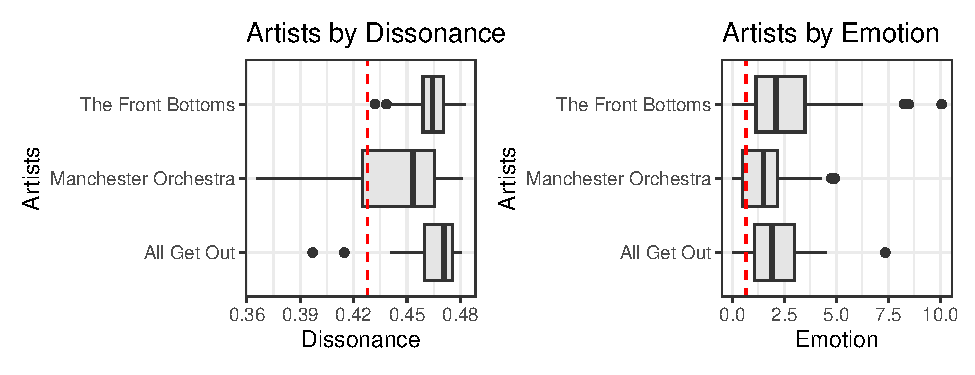
\includegraphics[width=\maxwidth]{figure/unnamed-chunk-3-1} 
\end{knitrout}

\begin{multicols}{2} 
We can now answer the question at hand for this lab, who contributed more to the song ``Allentown", Manchester Orchestra; The Front Bottoms; or All Get Out? With the data collection/extraction, data cleaning, and data summarizing/analysis we did earlier, we were able to derive a couple of figures which should allow us to answer the question. The results of our data analysis are shown above. The table we made using xtables \citep{xtable} figure above illustrates the in range, outlying, and out of range song traits for each artist in a numerical form, we got this from our summarized data frame. The next three column plots are the graphical representation of our table, which help us compare the magnitude of contribution each band had on ``Allentown" and allows us to compare artists easier. The last two plots are the box plots from the selected features we chose earlier in our first data extraction. This will serve as additional supporting evidence for our results. 



\columnbreak
\section{Discussion}
With the creation of our plots and tables, we can now accurately rank the artists in terms of contribution. Based on the table and the three corresponding column plots, it seems that Manchester Orchestra has the greater contribution on the song ``Allentown"! Manchester Orchestra has the most in range song traits while numbering less in outlying and out of range song traits in comparison to the other artists. All Get Out is the second biggest contributor since it has less in range song traits against Manchester Orchestra but more against The Front Bottoms. This would put The Front Bottoms as the smallest contributor to ``Allentown". These results are also reinforced by the select features we chose for box plot analysis. The red line on the box plots mark the song trait value for ``Allentown". As seen on the plots, ``Allentown" falls much more in range to the Manchester Orchestra box plots than the other two artists. Thus, the biggest contributor on ``Allentown" is Manchester Orchestra!

%%%%%%%%%%%%%%%%%%%%%%%%%%%%%%%%%%%%%%%%%%%%%%%%%%%%%%%%%%%%%%%%%%%%%%%%%%%%%%%%%%%%%%%%%%%%%%%%%%%%%%%%%%%%%%%%%%%%%
%Bibliography
%%%%%%%%%%%%%%%%%%%%%%%%%%%%%%%%%%%%%%%%%%%%%%%%%%%%%%%%%%%%%%%%%%%%%%%%%%%%%%%%%%%%%%%%%%%%%%%%%%%%%%%%%%%%%%%%%%%%%
\vspace{2em}
\begin{footnotesize}
\bibliography{bibliography.bib}
\end{footnotesize}

\end{multicols}

\end{document}
